
%% bare_conf.tex
%% V1.4b
%% 2015/08/26
%% by Michael Shell
%% See:
%% http://www.michaelshell.org/
%% for current contact information.
%%
%% This is a skeleton file demonstrating the use of IEEEtran.cls
%% (requires IEEEtran.cls version 1.8b or later) with an IEEE
%% conference paper.
%%
%% Support sites:
%% http://www.michaelshell.org/tex/ieeetran/
%% http://www.ctan.org/pkg/ieeetran
%% and
%% http://www.ieee.org/

%%*************************************************************************
%% Legal Notice:
%% This code is offered as-is without any warranty either expressed or
%% implied; without even the implied warranty of MERCHANTABILITY or
%% FITNESS FOR A PARTICULAR PURPOSE! 
%% User assumes all risk.
%% In no event shall the IEEE or any contributor to this code be liable for
%% any damages or losses, including, but not limited to, incidental,
%% consequential, or any other damages, resulting from the use or misuse
%% of any information contained here.
%%
%% All comments are the opinions of their respective authors and are not
%% necessarily endorsed by the IEEE.
%%
%% This work is distributed under the LaTeX Project Public License (LPPL)
%% ( http://www.latex-project.org/ ) version 1.3, and may be freely used,
%% distributed and modified. A copy of the LPPL, version 1.3, is included
%% in the base LaTeX documentation of all distributions of LaTeX released
%% 2003/12/01 or later.
%% Retain all contribution notices and credits.
%% ** Modified files should be clearly indicated as such, including  **
%% ** renaming them and changing author support contact information. **
%%*************************************************************************


% *** Authors should verify (and, if needed, correct) their LaTeX system  ***
% *** with the testflow diagnostic prior to trusting their LaTeX platform ***
% *** with production work. The IEEE's font choices and paper sizes can   ***
% *** trigger bugs that do not appear when using other class files.       ***                          ***
% The testflow support page is at:
% http://www.michaelshell.org/tex/testflow/



\documentclass[conference]{IEEEtran}
% Some Computer Society conferences also require the compsoc mode option,
% but others use the standard conference format.
%
% If IEEEtran.cls has not been installed into the LaTeX system files,
% manually specify the path to it like:
% \documentclass[conference]{../sty/IEEEtran}





% Some very useful LaTeX packages include:
% (uncomment the ones you want to load)


% *** MISC UTILITY PACKAGES ***
%
%\usepackage{ifpdf}
% Heiko Oberdiek's ifpdf.sty is very useful if you need conditional
% compilation based on whether the output is pdf or dvi.
% usage:
% \ifpdf
%   % pdf code
% \else
%   % dvi code
% \fi
% The latest version of ifpdf.sty can be obtained from:
% http://www.ctan.org/pkg/ifpdf
% Also, note that IEEEtran.cls V1.7 and later provides a builtin
% \ifCLASSINFOpdf conditional that works the same way.
% When switching from latex to pdflatex and vice-versa, the compiler may
% have to be run twice to clear warning/error messages.






% *** CITATION PACKAGES ***
%
\usepackage{cite}
% cite.sty was written by Donald Arseneau
% V1.6 and later of IEEEtran pre-defines the format of the cite.sty package
% \cite{} output to follow that of the IEEE. Loading the cite package will
% result in citation numbers being automatically sorted and properly
% "compressed/ranged". e.g., [1], [9], [2], [7], [5], [6] without using
% cite.sty will become [1], [2], [5]--[7], [9] using cite.sty. cite.sty's
% \cite will automatically add leading space, if needed. Use cite.sty's
% noadjust option (cite.sty V3.8 and later) if you want to turn this off
% such as if a citation ever needs to be enclosed in parenthesis.
% cite.sty is already installed on most LaTeX systems. Be sure and use
% version 5.0 (2009-03-20) and later if using hyperref.sty.
% The latest version can be obtained at:
% http://www.ctan.org/pkg/cite
% The documentation is contained in the cite.sty file itself.


\usepackage{graphicx}



% *** GRAPHICS RELATED PACKAGES ***
%
\ifCLASSINFOpdf
  % \usepackage[pdftex]{graphicx}
  % declare the path(s) where your graphic files are
  % \graphicspath{{../pdf/}{../jpeg/}}
  % and their extensions so you won't have to specify these with
  % every instance of \includegraphics
  % \DeclareGraphicsExtensions{.pdf,.jpeg,.png}
\else
  % or other class option (dvipsone, dvipdf, if not using dvips). graphicx
  % will default to the driver specified in the system graphics.cfg if no
  % driver is specified.
  % \usepackage[dvips]{graphicx}
  % declare the path(s) where your graphic files are
  % \graphicspath{{../eps/}}
  % and their extensions so you won't have to specify these with
  % every instance of \includegraphics
  % \DeclareGraphicsExtensions{.eps}
\fi
% graphicx was written by David Carlisle and Sebastian Rahtz. It is
% required if you want graphics, photos, etc. graphicx.sty is already
% installed on most LaTeX systems. The latest version and documentation
% can be obtained at: 
% http://www.ctan.org/pkg/graphicx
% Another good source of documentation is "Using Imported Graphics in
% LaTeX2e" by Keith Reckdahl which can be found at:
% http://www.ctan.org/pkg/epslatex
%
% latex, and pdflatex in dvi mode, support graphics in encapsulated
% postscript (.eps) format. pdflatex in pdf mode supports graphics
% in .pdf, .jpeg, .png and .mps (metapost) formats. Users should ensure
% that all non-photo figures use a vector format (.eps, .pdf, .mps) and
% not a bitmapped formats (.jpeg, .png). The IEEE frowns on bitmapped formats
% which can result in "jaggedy"/blurry rendering of lines and letters as
% well as large increases in file sizes.
%
% You can find documentation about the pdfTeX application at:
% http://www.tug.org/applications/pdftex





% *** MATH PACKAGES ***
%
%\usepackage{amsmath}
% A popular package from the American Mathematical Society that provides
% many useful and powerful commands for dealing with mathematics.
%
% Note that the amsmath package sets \interdisplaylinepenalty to 10000
% thus preventing page breaks from occurring within multiline equations. Use:
%\interdisplaylinepenalty=2500
% after loading amsmath to restore such page breaks as IEEEtran.cls normally
% does. amsmath.sty is already installed on most LaTeX systems. The latest
% version and documentation can be obtained at:
% http://www.ctan.org/pkg/amsmath





% *** SPECIALIZED LIST PACKAGES ***
%
%\usepackage{algorithmic}
% algorithmic.sty was written by Peter Williams and Rogerio Brito.
% This package provides an algorithmic environment fo describing algorithms.
% You can use the algorithmic environment in-text or within a figure
% environment to provide for a floating algorithm. Do NOT use the algorithm
% floating environment provided by algorithm.sty (by the same authors) or
% algorithm2e.sty (by Christophe Fiorio) as the IEEE does not use dedicated
% algorithm float types and packages that provide these will not provide
% correct IEEE style captions. The latest version and documentation of
% algorithmic.sty can be obtained at:
% http://www.ctan.org/pkg/algorithms
% Also of interest may be the (relatively newer and more customizable)
% algorithmicx.sty package by Szasz Janos:
% http://www.ctan.org/pkg/algorithmicx




% *** ALIGNMENT PACKAGES ***
%
%\usepackage{array}
% Frank Mittelbach's and David Carlisle's array.sty patches and improves
% the standard LaTeX2e array and tabular environments to provide better
% appearance and additional user controls. As the default LaTeX2e table
% generation code is lacking to the point of almost being broken with
% respect to the quality of the end results, all users are strongly
% advised to use an enhanced (at the very least that provided by array.sty)
% set of table tools. array.sty is already installed on most systems. The
% latest version and documentation can be obtained at:
% http://www.ctan.org/pkg/array


% IEEEtran contains the IEEEeqnarray family of commands that can be used to
% generate multiline equations as well as matrices, tables, etc., of high
% quality.




% *** SUBFIGURE PACKAGES ***
%\ifCLASSOPTIONcompsoc
%  \usepackage[caption=false,font=normalsize,labelfont=sf,textfont=sf]{subfig}
%\else
%  \usepackage[caption=false,font=footnotesize]{subfig}
%\fi
% subfig.sty, written by Steven Douglas Cochran, is the modern replacement
% for subfigure.sty, the latter of which is no longer maintained and is
% incompatible with some LaTeX packages including fixltx2e. However,
% subfig.sty requires and automatically loads Axel Sommerfeldt's caption.sty
% which will override IEEEtran.cls' handling of captions and this will result
% in non-IEEE style figure/table captions. To prevent this problem, be sure
% and invoke subfig.sty's "caption=false" package option (available since
% subfig.sty version 1.3, 2005/06/28) as this is will preserve IEEEtran.cls
% handling of captions.
% Note that the Computer Society format requires a larger sans serif font
% than the serif footnote size font used in traditional IEEE formatting
% and thus the need to invoke different subfig.sty package options depending
% on whether compsoc mode has been enabled.
%
% The latest version and documentation of subfig.sty can be obtained at:
% http://www.ctan.org/pkg/subfig




% *** FLOAT PACKAGES ***
%
%\usepackage{fixltx2e}
% fixltx2e, the successor to the earlier fix2col.sty, was written by
% Frank Mittelbach and David Carlisle. This package corrects a few problems
% in the LaTeX2e kernel, the most notable of which is that in current
% LaTeX2e releases, the ordering of single and double column floats is not
% guaranteed to be preserved. Thus, an unpatched LaTeX2e can allow a
% single column figure to be placed prior to an earlier double column
% figure.
% Be aware that LaTeX2e kernels dated 2015 and later have fixltx2e.sty's
% corrections already built into the system in which case a warning will
% be issued if an attempt is made to load fixltx2e.sty as it is no longer
% needed.
% The latest version and documentation can be found at:
% http://www.ctan.org/pkg/fixltx2e


%\usepackage{stfloats}
% stfloats.sty was written by Sigitas Tolusis. This package gives LaTeX2e
% the ability to do double column floats at the bottom of the page as well
% as the top. (e.g., "\begin{figure*}[!b]" is not normally possible in
% LaTeX2e). It also provides a command:
%\fnbelowfloat
% to enable the placement of footnotes below bottom floats (the standard
% LaTeX2e kernel puts them above bottom floats). This is an invasive package
% which rewrites many portions of the LaTeX2e float routines. It may not work
% with other packages that modify the LaTeX2e float routines. The latest
% version and documentation can be obtained at:
% http://www.ctan.org/pkg/stfloats
% Do not use the stfloats baselinefloat ability as the IEEE does not allow
% \baselineskip to stretch. Authors submitting work to the IEEE should note
% that the IEEE rarely uses double column equations and that authors should try
% to avoid such use. Do not be tempted to use the cuted.sty or midfloat.sty
% packages (also by Sigitas Tolusis) as the IEEE does not format its papers in
% such ways.
% Do not attempt to use stfloats with fixltx2e as they are incompatible.
% Instead, use Morten Hogholm'a dblfloatfix which combines the features
% of both fixltx2e and stfloats:
%
% \usepackage{dblfloatfix}
% The latest version can be found at:
% http://www.ctan.org/pkg/dblfloatfix


\usepackage{listings}

% *** PDF, URL AND HYPERLINK PACKAGES ***
%
%\usepackage{url}
% url.sty was written by Donald Arseneau. It provides better support for
% handling and breaking URLs. url.sty is already installed on most LaTeX
% systems. The latest version and documentation can be obtained at:
% http://www.ctan.org/pkg/url
% Basically, \url{my_url_here}.




% *** Do not adjust lengths that control margins, column widths, etc. ***
% *** Do not use packages that alter fonts (such as pslatex).         ***
% There should be no need to do such things with IEEEtran.cls V1.6 and later.
% (Unless specifically asked to do so by the journal or conference you plan
% to submit to, of course. )


% correct bad hyphenation here
\hyphenation{op-tical net-works semi-conduc-tor}


\begin{document}
%
% paper title
% Titles are generally capitalized except for words such as a, an, and, as,
% at, but, by, for, in, nor, of, on, or, the, to and up, which are usually
% not capitalized unless they are the first or last word of the title.
% Linebreaks \\ can be used within to get better formatting as desired.
% Do not put math or special symbols in the title.
\title{Examining Security Issues in Dolphin Netplay}


% author names and affiliations
% use a multiple column layout for up to three different
% affiliations
\author{\IEEEauthorblockN{Austin Taghavi}
\IEEEauthorblockA{Department of Computer Science and Engineering\\
Texas A\&M University\\
College Station, TX\\
Email: austintaghavi@gmail.com}
\and
\IEEEauthorblockN{Philip Van Ruitenbeek}
\IEEEauthorblockA{Department of Computer Science and Engineering\\
Texas A\&M University\\
College Station, TX\\
Email: philipvr@gmail.com}
}

% conference papers do not typically use \thanks and this command
% is locked out in conference mode. If really needed, such as for
% the acknowledgment of grants, issue a \IEEEoverridecommandlockouts
% after \documentclass


% make the title area
\maketitle

% As a general rule, do not put math, special symbols or citations
% in the abstract
%\begin{abstract}
%The abstract goes here.
%\end{abstract}

% no keywords




% For peer review papers, you can put extra information on the cover
% page as needed:
% \ifCLASSOPTIONpeerreview
% \begin{center} \bfseries EDICS Category: 3-BBND \end{center}
% \fi
%
% For peerreview papers, this IEEEtran command inserts a page break and
% creates the second title. It will be ignored for other modes.
\IEEEpeerreviewmaketitle

\begin{abstract}
   Online gaming is no longer simply a past-time for the youth; it is not only a large industry, but also a career for many.
   Because of this, online gaming security is becoming more and more important.
   Hacking online games can amount to a serious offense if it is used to skew the results of games played for money.
   In this report, we explore the security concerns of Super Smash Bros Melee, as played through Netplay.
   We explore methods of cheating within the game, performing malicious activity, as well as possible security measures to address these problems.
\end{abstract}

\section{Introduction}
Online gaming is as popular as it has ever been, and only continues to grow. 
With the advent of eSports, we are seeing competitive video gaming turn into a legitimate industry. Video games are played for fun, but they are also played for sport and, in some cases, as a career. This changes security issues and cheating in online gaming from an annoyance to a serious issue. 
Cheating in online gaming that results in a change in the outcome of the game can have financial implications and can be a serious crime.
	
One such eSport is the Super Smash Bros franchise, from Nintendo.
This is considered by many to be the first eSport, as the competitive Super Smash Bros scene emerged before the game was playable online.
While newest installations of Super Smash Bros have online support through Nintendo, older versions do not.
In particular, we are concerned with Super Smash Bros Melee, which we will refer to as SSBM throughout this report.
The competitive community for SSBM began with groups of people meeting in person and holding tournaments.
However, in recent years, ways of playing the game online have emerged.
Dolphin is a Gamecube emulator for Windows, which provides a system called NetPlay for playing certain Gamecube games online.
Players can meet in online, on sites such as Anther's Ladder.
These sites provide a platform for players to meet eachother and coordinate games.
Tournaments are also organized via websites such as these, and many of these such tournaments are played for prize money. 
Thus, security implications are very serious for this game.

We wish to explore the security issues with NetPlay for Dolphin, in particular how they pertain to SSBM. 
Our analysis will be threefold: (1) Cheating at SSBM through NetPlay for Dolphin, (2) Malicious activity via the connection provided by NetPlay, and (3) possible solutions for the issues we find.


\section{Related Work}
The online PC gaming in the U.S. is a multi-billion dollar industry \cite{takahashi15}. When online gamers encounter cheaters, they may feel that the game is ruined and may give up on playing the game \cite{yan02}. 

In Blizzard's World of Warcraft (WoW) players may sell virtual items for real-world money through middle market companies that allow for the currency exchange \cite{mcgraw09}. This enables cheating to be monetized, thereby incentivizing hackers to find vulnerabilities in the game which can be used to gain an advantage over other players.

Online games are massively distributed systems. Game designers often place to much essential functionality in the game's client software on the machines of potential hackers \cite{mcgraw09}. Instead critical game functionality should be placed within trusted game servers.

Online gaming is the most successful software industry in Asia and has led to a rapid increase in cyber-criminal activity in Taiwan \cite{chen04}. 

Steam, a popular online game platform, reported that 77,000 accounts are hijacked and pillaged each month \cite{steam15}. It was later found by \cite{pontiroli16} that malware had been developed to steal Steam user credentials.

By using a time series based user modeling approach in \cite{oh12} compromised accounts can be automatically detected in Massively Multi-player Online Role Playing Games. \cite{chen07} found that idle time distribution is a representative feature of game players.

\section{Research Areas}
We want to explore vulnerabilities and exploits of these vulnerabilities in Netplay for Dolphin.
There are many types of security vulnerability, so we will split the research into 4 research areas:
\vspace{0.5cm}
\begin{enumerate}  
\item Eavesdropping
\item Network traffic spoofing
\item Piggybacking
\item Solutions
\end{enumerate}
\vspace{0.5cm}

\subsection{Eavesdropping}
This type of vulnerability refers to the malicious activity that an attacker could perform just by listening to network traffic.
This mainly amounts to an attacker getting private information about victims by listening to network traffic.
In general, this type of attack requires the attacker to be on the same network as one or more victims.

\subsection{Network traffic spoofing}
This type of vulnerability refers to when an attacker "spoofs" network traffic to change the course of a game or chat session.
One possibility is for an attacker to "spoof" traffic to send controller input from one player to the server, in order to cheat at the game and make a specific player win or lose.
Another possibility is for an attacker to spoof packets to change the game settings for one player, to give a specific player an unfair advantage.
Again, this type of vulnerability generally requires the attacker to have access to the network of one of more player.

\subsection{Piggybacking}
In this context, we are using "piggybacking" to mean an attack in which the attacker modifies the source code of Dolphin to include some kind of malicious code.
The attacker then distributes their new compiled app, and victims download the attacker's version of Dolphin, thinking that it is a legitimate version of Dolphin.
The victim is then vulnerable to whatever malicious code the attacker included.
One example is the attacker distributing a Dolphin binary that sends out personal or sensitive data to their own private server.

\subsection{Solutions}
We will also discuss and explore possible solutions to the vulnerabilities and exploits that we find.
While vulnerabilities always exist, we believe that we can provide valuable insight into various ways that security in Dolphin and NetPlay can be improved. 
We will suggest solutions to vulnerabilities for both the user and for the developers of Dolphin.

\section{NetPlay Overview}
NetPlay is an online gaming platform that is provided by the Dolphin emulator. It provides a way for players using the emulator to play games against each other via the internet. These games do not necessarily need to have had online play originally implemented. 

There are two different ways in which users can communicate with one another to establish a game.
\vspace{0.5cm}
\begin{enumerate}  
\item Direct Connection
\item Traversal Server
\end{enumerate}
\vspace{0.5cm}
For both of these connection types, the flow of communication is the same. It consists of the following:

\begin{enumerate}  
\item One user "hosts" the game, and communicates a GUID for the game to the other player
\item The other user(s) "connects" to the session.
\item The host decides when to start the game.
\item Both (or all) sides communicate their controller input for the game to take place.
\end{enumerate}
\vspace{0.cm}

An example sequence diagram for a direct connection is provided below:
\begin{center}
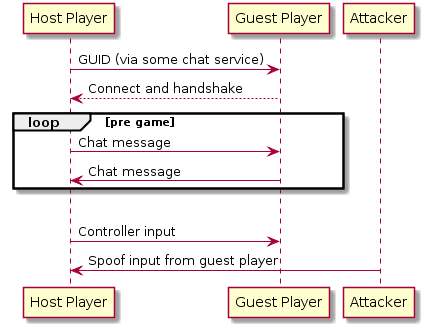
\includegraphics[width=9cm]{Figures/Basic_Sequence}
\end{center}
\vspace{0.3cm}
And the equivalent diagram for the traversal server:
\begin{center}
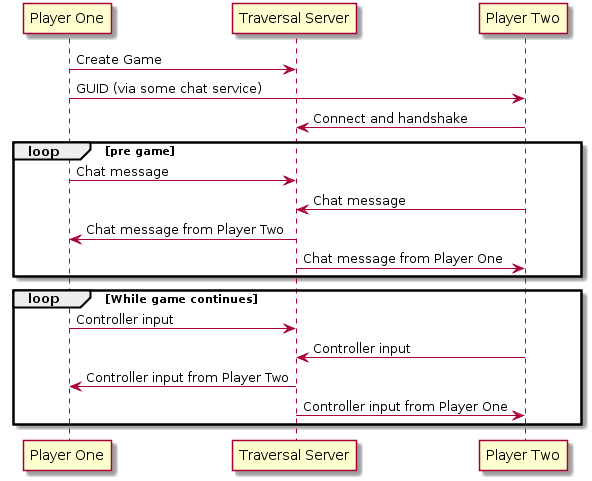
\includegraphics[width=9cm]{Figures/Sequence_Traversal}
\end{center}
\vspace{0.3cm}



\section{ Networking Traffic Spoofing }

\section{Source Code Analysis}
The Dolphin emulator project has been around since 2003.
The project was made open source in 2008.
The source code for the Dolphin emulator is available online on github \cite{github-dolphin}.
Maintenance and additions to the project are a community effort, relying on many coders working on the project as a labor of love.
As part of our research into the security issues with Netplay and Dolphin in general, in this section we present our finding from analyzing the source code of Dolphin.
We present an overview of the structure of Netplay, as well as our thoughts on some of the vulnerabilities that are apparent through looking at the source code.
The Dolphin emulator project consists of upwards of 800,000 lines of code.
Most of the code is written in C++, and the project is compilable on Windows, Linux, and Mac OS X.

\subsection{ NetPlay Structure }
There are two primary actors in a Netplay session, namely the client and server.
Each player in the game is represented as a "client" in the session.
In addition, the "hosting" player also runs a server.
Data is sent from the clients to the server, who forwards the data to the appropriate clients.
Some data is sent only from the server, such as the signal to start or stop a game.
In general, changes are made locally and packets are sent out to notify the other clients in the game.
For instance, controller input is sent straight to the local emulator, and then other clients are notified.
In a sense, there is very little syncing through the server.
When a packet is received by the client or server, the client/server decides where to send the data based on which type of message it is.
For example: a chat message is simply displayed in the chat window by calling a UI function, and controller input is actually forwarded to the emulator to be input.

\subsection{Data types}
The following are types of packets that are sent by client or server:

\vspace{0.5cm}
\begin{enumerate}  
\item Chat message
\item Gamecube controller input
\item Wiimote controller input
\item Player join/leave
\item Change game
\item Start game
\item Stop game
\item Ping
\item Compute MD5 hash of game
\item Change game settings
\end{enumerate}
\vspace{0.5cm}

The MD5 hash is computed to make sure that clients are using the same version of a game, to minimize possible issues with that.
There is no encryption on any of the data sent.

\subsection{Possible vulnerabilities}
Through our source code analysis, we found numerous vulnerabilities that require different kinds of exploits. 
Primarily, there is no encryption or sequence number validation. 
This makes Netplay a much easier target for network and packet spoofing attacks than if they had used encryption.
It appears that packets spoofed from one client to the server, or from the server to a client, will be taken in by Netplay, and the data will be used.
There is little to no verification of the data sent. 
This lack of encryption also means that chat messages are sent in plantext.
This presents a security issue because anyone on the network of any of the clients will be able to listen to the traffic and read chat messages in plain text.

The lack of syncing provides other opportunities for attackers.
Primarily, it provides an opportunity for attackers to spoof or fake messages without the "sender" knowing that it was sent.
For example, an attacker could implement a "piggybacking" attack in which phishing messages are sent without one party even being aware that the messages are sent.
This would be particularly effective, because one party would believe that their friend or trusted person was sending these messages, while the supposed "sender" is never even aware that the messages are sent.


\section{Eavesdropping}
Our first task was to monitor traffic during a game of SSBM via NetPlay. 
The goal of this is to capture and observe network traffic to analyze security vulnerabilities. 
From there we will design and explore possible exploits.
Our experiment here is simple: Play a game of SSBM between two hosts via NetPlay, and monitor the network traffic during the game.

For monitoring, we used the tool "Wireshark" to capture network traffic. During our capture, we used the following filter:

$ ( ip.src == IP_1 \&\& ip.dst == IP_2 ) || (ip.src == IP_2 \&\& ip.dst == IP_1) \&\& udp) $

\vspace{0.3cm}
This filter allowed us to only look at traffic that is to and from the two IP addresses that we used, and only UDP traffic of that.
Initially the traffic was numerous and overwhelming.
We were able to do shorter captures of different stages of the game to narrow down the traffic and more closely associate it with different actions in the game.
For this, we broke the game down into two stages:
\begin{enumerate}  
\item Initial handshake and pre-game
\item During game communication
\end{enumerate}
\vspace{0.5cm}

Some of the initial handshake data is somewhat indecipherable to us. 
However, the pre-game client allows users to "chat" with eachother, and this is easily decipherable. 
An example of such a packet is provided below:
\vspace{0.5cm}
\begin{center}
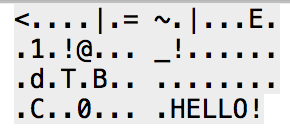
\includegraphics[width=4cm]{Figures/Packet2}
\end{center}
\vspace{0.5cm}

As the reader can easily see, the chat messages are sent in plaintext.
This is unsafe, as anyone on the network can listen to the traffic and see what messages are sent.
Because many players will play games via NetPlay with trusted friends, they may be inclined to share information with them that most would consider sensitive.
This would be unwise, because this information can easily be seen by anyone on the network.

For the actual game communication, it is our analysis that the games send "controller input" back and forth to establish the game. An example of such a packet is provided below:
\vspace{0.5cm}
\begin{center}
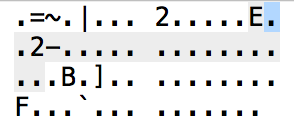
\includegraphics[width=4cm]{Figures/Packet}
\end{center}
\vspace{0.5cm}

Each of these UDP packets contains data about a single controller input.
The payload data contains values for each input on the controller: binary values for buttons and real values for the joysticks.
This data is not of much use to an attacker if they are simply listening to the traffic, as it is hard to consider this information sensitive. 

\section{Network traffic spoofing}
In this section, we explore many different network spoofing attacks.
The common factor in all of these attacks is that the attacker is on the same network as one of the players of NetPlay, and spoofs network traffic to have some malicious effect.
Some of the attacks attempt to effect gameplay to "cheat" at a game, while others have a more general malicious purpose of just sending chat messages from another person.
\subsection{Tools used for spoofing}
To implement these attacks, we need to be able to spoof packets and send them out on a network. We describe some of the tools that we used below.

We use a python tool and library called \textbf{scapy} to construct packets, edit pcap files, and send packets out over a network. 
Particularly, we  need to construct UDP packets and be able to "spoof" the sender address of such packets.
By this, we mean that we need to be able to indicate that a packet is coming from another host.
We have chosen to implement a simple packet spoofer in Python, and use this to perform the attack.
A small sample code snippet is provided below:
\vspace{0.3cm}
\begin{lstlisting}[language=Python]
spoofed_packet = 
   IP(src=src_IP, dst=dst_IP) / 
   UDP(sport=src_port, dport=dst_port) / 
   payload
send(spoofed_packet)
\end{lstlisting}
\vspace{0.3cm}
The \textbf{scapy} library makes the construction and sending of spoofed packets very simple.
Another usecase for \textbf{scapy} is to take in a pcap file containing captured network data, and make some edits to it.
Provided below is a code snippet of \textbf{scapy} code to take in a pcap file, and generate new IPV4 identification fields, recompute checksums, and save the result in a new pcap file.
\vspace{0.3cm}
\begin{lstlisting}[language=Python]
pktdump = PcapWriter("output.pcap",
	append=True, 
	sync=True)
pkts=rdpcap("input.pcap")
for pkt in pkts:
	#generate new ID field
	pkt[IP].id = random.randint(1000,30000)  
	del pkt[IP].chksum
	del pkt[UDP].chksum
	pktdump.write(pkt)
\end{lstlisting}
\vspace{0.3cm}

In addition to \textbf{scapy}, we also used a tool to make playing our pcap files easier.
For this, we used a very commonly used tool called \textbf{PlayCap}. 
\textbf{PlayCap} allowed us to "play" the modified pcap files that we created using \textbf{scapy} over the network.
To be clear: given a pcap file, \textbf{PlayCap}  will send all of the packets over the network, exactly as they are defined in the pcap file.

\subsection{Controller input attack}
For this experiment, we will first begin a game  via NetPlay between two hosts.
We will then use a third party computer to spoof packets to interfere with the game.
The third party will spoof packets "pretending" to be one of the hosts (the victim, in this case), and sending facetious and malicious data.
An example sequence diagram for a direct connection is provided below:
\begin{center}
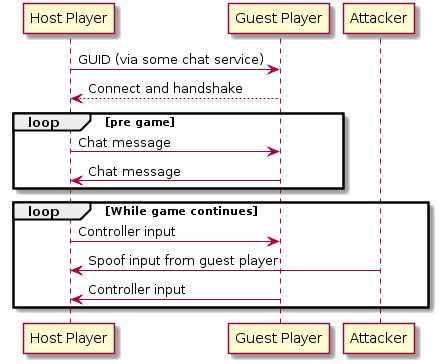
\includegraphics[width=8cm]{Figures/Sequence1}
\end{center}
\vspace{0.5cm}
And the equivalent diagram for a traversal server is:
\begin{center}
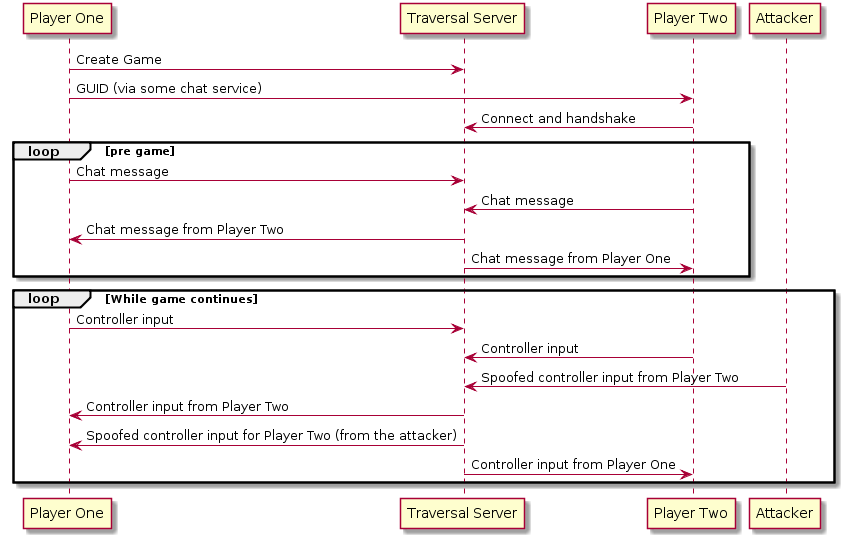
\includegraphics[width=8cm]{Figures/Sequence2}
\end{center}

Because it was not immediately clear to us how these packets would look, we first listened to traffic and picked out controller input packets. 
We singled out controller input packets by doing different controller input patters, and analyzing the resulting traffic.
Once we singled out a specific controller input packet that we wanted to spoof, we captured the traffic and saved the results in a pcap file.
We then used \textbf{scapy} to modify this file by changing the IPV4 identification numbers, and recomputing checksums.
Then, we used \textbf{PlayCap} to send the newly created pcap file out over the network.
The intended result of this would be that the controller input would be spoofed, and we would see the result in the game. 

\subsection {Spoofing chat messages}

\subsection {Spoofing game settings}

\subsection{Drawbacks}

\section{Piggybacking}
In this section we discuss various attack methods that take advantage of the open source nature of the Dolphin emulator.
In particular, we detail attacks that involve the attacker modifying the source code of Dolphin, recompiling the project, and distributing their modified binaries.
We discuss two attacks in detail, and then give an overview of the possibilities for other attacks, and conclude with some drawbacks to this method of attack.
\subsection{Stealing user info}
The NetPlay portion of the Dolphin emulator has access to some sensitive user information.
It has access to all of the player's IP addresses, as well as their player info, and all of their chat messages.
It is clear that this is information that an attacker may want to get ahold of.
We found the relevant code in the Dolphin project for this attack, and implemented the attack. 
Below you can see a code snippet that contains the malicious code:

\vspace{0.5cm}
\begin{center}
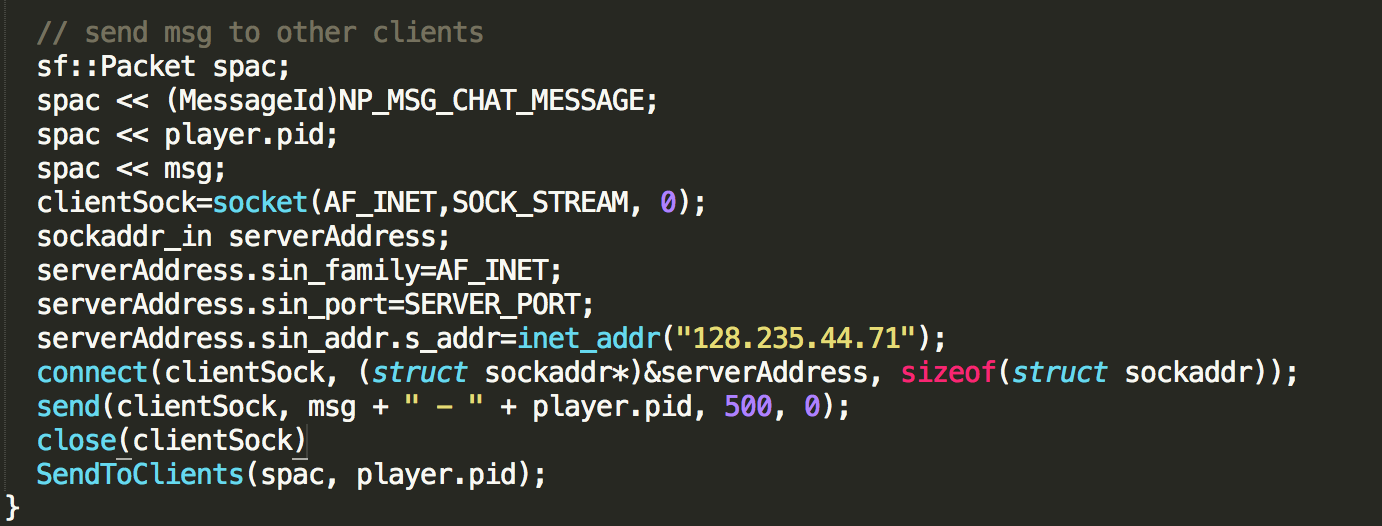
\includegraphics[width=9cm]{Figures/Stealing}
\end{center}
\vspace{0.5cm}

This code intercepts chat messages as they are being sent to other clients, and sends them out to a private server, owned by the attacker.
Other than monitoring their own network traffic, the victim will have no way of knowing this is happening.
This malicious code works as intended.
\subsection{Phishing}

\subsection{Other possibilities}
\subsection{Drawbacks}

\section{Solutions and Suggestions}

\section{Conclusion}




% trigger a \newpage just before the given reference
% number - used to balance the columns on the last page
% adjust value as needed - may need to be readjusted if
% the document is modified later
%\IEEEtriggeratref{8}
% The "triggered" command can be changed if desired:
%\IEEEtriggercmd{\enlargethispage{-5in}}

% references section

% can use a bibliography generated by BibTeX as a .bbl file
% BibTeX documentation can be easily obtained at:
% http://mirror.ctan.org/biblio/bibtex/contrib/doc/
% The IEEEtran BibTeX style support page is at:
% http://www.michaelshell.org/tex/ieeetran/bibtex/
\bibliographystyle{IEEEtran}
% argument is your BibTeX string definitions and bibliography database(s)
\bibliography{bib}
%
% <OR> manually copy in the resultant .bbl file
% set second argument of \begin to the number of references
% (used to reserve space for the reference number labels box)
%\begin{thebibliography}{1}
%
%\bibitem{IEEEhowto:kopka}
%H.~Kopka and P.~W. Daly, \emph{A Guide to \LaTeX}, 3rd~ed.\hskip 1em plus
%  0.5em minus 0.4em\relax Harlow, England: Addison-Wesley, 1999.
%
%\end{thebibliography}




% that's all folks
\end{document}


